%
% file: localoperator.tex
% author: Victor Brena
% description: Briefly describes properties of the local operator.
%

\chapter{Apéndice A}
\label{app:app01}

\textbf{Autenticación de acceso al API GitHub.} Existen tres formas de autenticación de acceso al API v3 de GitHub, ésto para evitar la salida de repositorios privados a usuarios no autorizados (\citeyear{ratelimit_github}).

\begin{enumerate}[1.]
    \item \textbf{\textit{Autenticación Básica}}. Permite realizar 60 peticiones por hora. El acceso puede ser solicitado vía ''usuario y contraseña''; donde el usuario y la contraseña asociados a una cuenta son enviados a través de la url.
\begin{center}
\small \texttt{ \$ curl -u <username>\space https://api.github.com/user}
\end{center}		    
   
    \item  \textbf{\textit{OAuth2 Token}}. Con ayuda de la interfaz de usuario en GitHub, se obtiene una llave llamada “Personal Access Token o OAuth Token” que será utilizada cómo contraseña al momento de solicitar el acceso al API a través de la url. 
         % A single figure
        \begin{figure}[H]
            \centering
            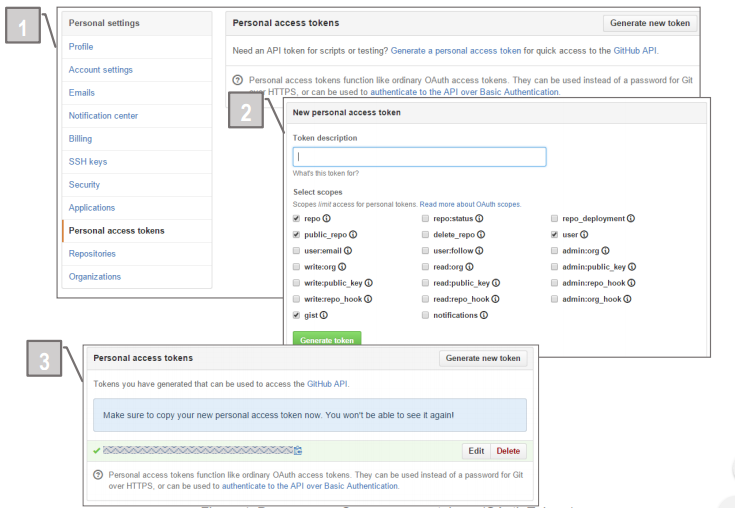
\includegraphics[height=0.4\textheight]{oauth_git}
            \mycaption[Proceso para crear un nuevo token (OAuth Token)]{Proceso para crear un nuevo token (OAuth Token).}
            \label{fig:RHP02}
        \end{figure}
        
Debido a que el proceso para crear un nuevo OAuth Token es realizado dentro de la plataforma GitHub es importante estar registrado para llevar a cabo las instrucciones mostradas en la Figura A.1, y que consisten en:
\begin{enumerate}[1.]
\item Hacer click sobre la opción ''Personal access tokens'' dentro del menú desplegado en el apartado de Configuración (Settings).
\item Dar click en el enlace ''Generate a personal access token'' y llenar el formato de permisos para la creación del token.
\item Luego de llenar el formato, hacer click sobre el botón "Generate token", el cual desplegará otra página que contiene el token de acceso OAuth.
\end{enumerate}
    
Para obtener acceso al API GitHub, el token OAuth generado puede ser enviado a través de las siguientes opciones:

    \begin{enumerate}[a)]
        \item Enviando token en el encabezado.
% * <alegarcia@uaz.edu.mx> 2016-11-07T17:18:15.436Z:
%
% > Enviado en un encabezado.
%
% Aquí qué es lo que se envía ? la petición de autenticación como encabezado? 
%
% ^.
\begin{center}
\small \texttt{ \$ curl -H ''Authorization: token OAUTH-TOKEN'' https://api.github.com}
\end{center}
        
        \item Enviando token como parámetro.
        
\begin{center}
\small \texttt{ \$ curl https://api.github.com/?access\_token=OAUTH-TOKEN}
\end{center}
        
        
    \end{enumerate}
    
    \item \textbf{\textit{OAuth2 Key/Secret}}. Ésta opción permite realizar 5000 peticiones por hora. La llave del cliente (key) y la llave secreta (secret) son asignadas a través del proceso de registro de una aplicación en GitHub.

 % A single figure
        \begin{figure}[H]
            \centering
            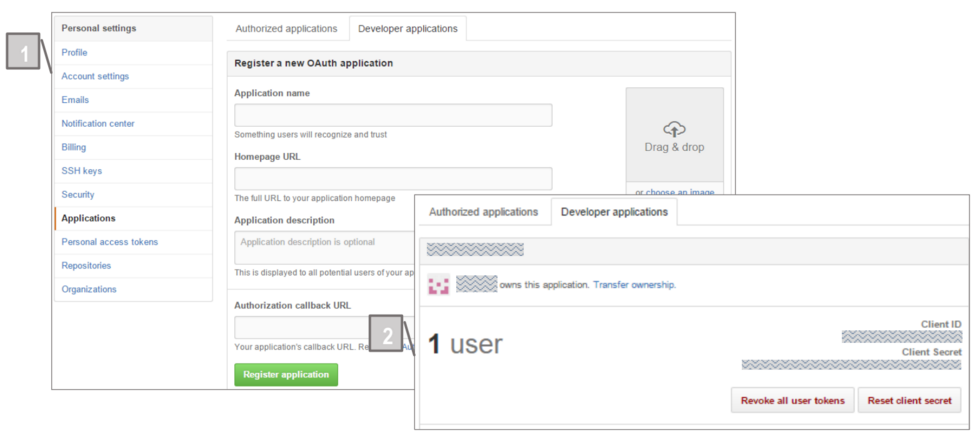
\includegraphics[height=0.25\textheight]{oauth2_git}
            \mycaption[Proceso de autenticación OAuth2 Key/Secret]{Proceso de autenticación OAuth2 Key/Secret}
            \label{fig:RHP02}
        \end{figure}
        
Como se puede observar en la Figura A.2, el proceso de autenticación OAuth2 es realizado sobre la interfaz de usuario de la plataforma GitHub, por ello es necesario contar con una cuenta dentro de ésta plataforma para llevar a cabo las siguientes instrucciones.

\begin{enumerate}[1.]
\item Dentro del apartado de ''Configuración (Settings)'' en GitHub, hacer click sobre la opción ''Applications''.
\item Dar click sobre el botón ''Register a new application'', llenar el formato de registro de la aplicación, y finalmente, hacer click sobre el botón ''Register application''.
\end{enumerate}

    
\end{enumerate}


\chapter{Apéndice B}
\label{app:app02}
% * <alegarcia@uaz.edu.mx> 2016-11-07T17:19:10.394Z:
%
% Agrega un título: Configuración para el API Twitter por ejemplo.....
%
% ^.
\textbf{Autenticación de acceso al API Twitter.} Antes de comenzar a describir el proceso de autenticación, es primordial contar con una cuenta en Twitter, ya que el acceso al API Twitter es por medio de las credenciales de autenticación (API key, API secret, Access token y Access token secret), que son obtenidas a través del sitio de desarrollo de Twitter (\citeauthor{oauth_twitter}, \citeyear{oauth_twitter}).

\begin{enumerate}[1.]
    \item Crear una cuenta de usuario de Twitter, en caso de no tener una. 
    \item Ir a \textit{https://apps.twitter.com/} y logearse con la cuenta usuario de Twitter. Éste paso le dará una cuenta de desarrollo bajo el mismo nombre que su cuenta de usuario en Twitter.
    \item Hacer Click en ''Create New App''.
    \item Llenar la forma, aceptar los términos, y hacer click en “Create your Twitter application”.
    \item En la siguiente página, hacer click sobre “Keys and Access Tokens”, y copiar el “API key” y “API secret”. 
    \item Deslizar hacia abajo y dar click en “Create my access token”, y copiar el “Access token” y “Access token secret”.
    
\end{enumerate}








